\begin{figure}
   \subcaptionbox
      {4 dependency relations}
      {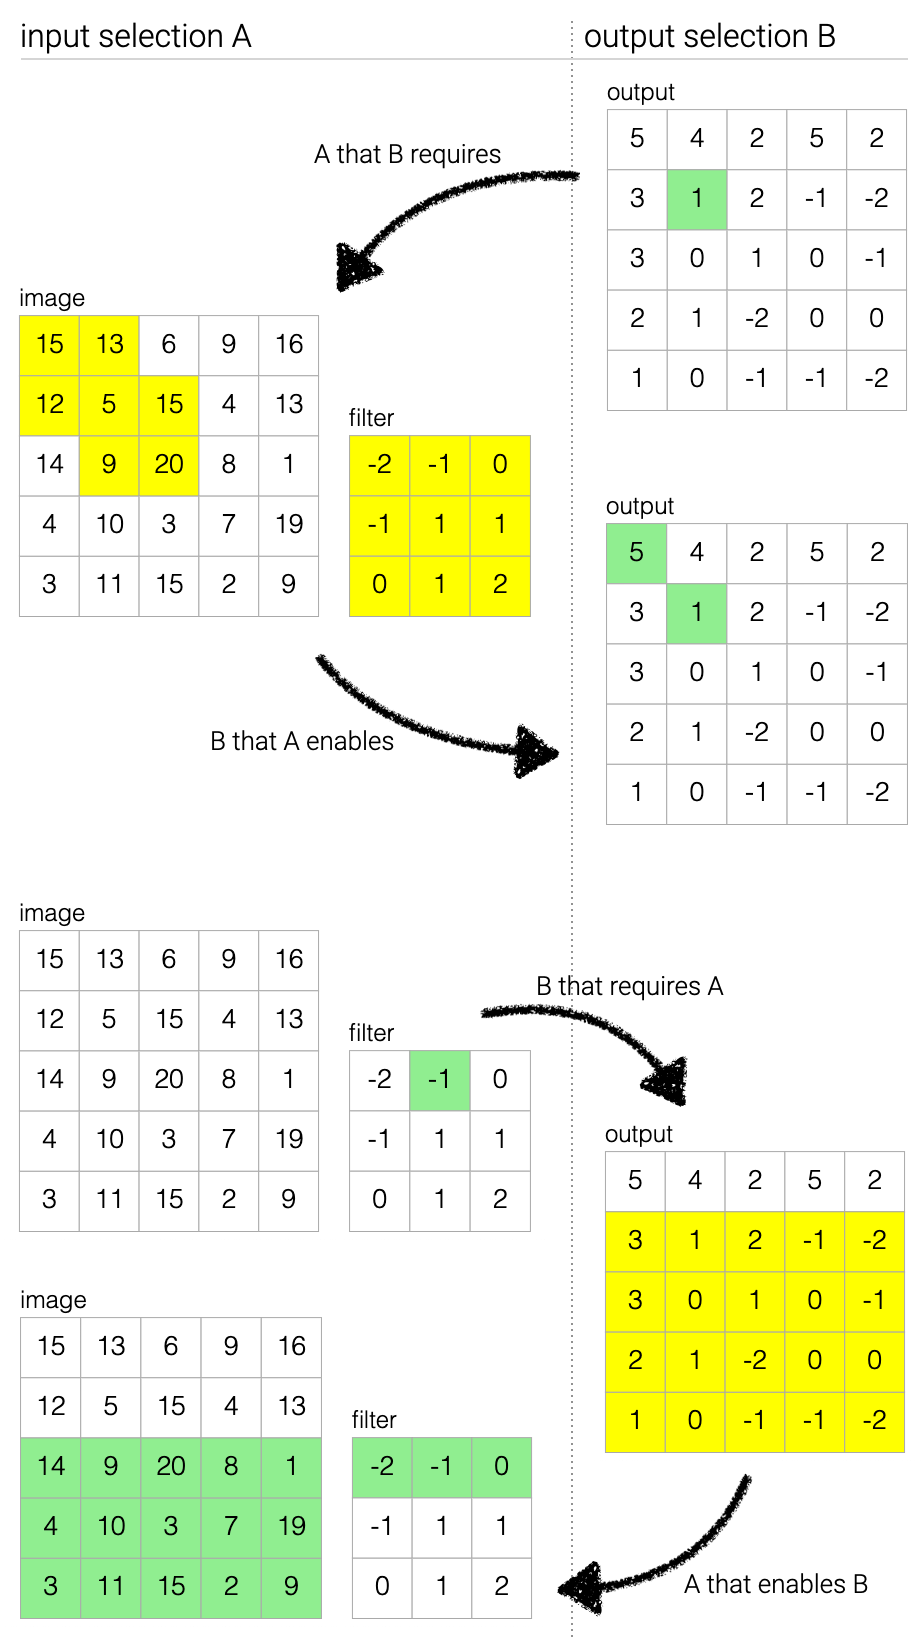
\includegraphics[scale=0.4]{fig/example/4-relations.png}}
   \subcaptionbox
      {Matrix convolution example}
      {
         \small
         \lstinputlisting[language=Fluid]{fluid/convolution.fld.mod}
%         \caption{Matrix convolution, with three methods for dealing with boundaries}
         \lstinputlisting[language=Fluid]{fluid/conv-extend.fld.mod}
%         \caption{Convolving example matrix with supplied filter and choice of boundary method}
      }
   \caption{TODO}
\end{figure}
